\documentclass[runningheads]{llncs}

\usepackage[utf8]{inputenc}
\usepackage[T1]{fontenc}
\usepackage[english]{babel}
\usepackage{graphicx}
\usepackage{booktabs}
\usepackage{amsmath}
\usepackage{url}
\usepackage{xcolor}
\usepackage{amssymb}
\usepackage{multirow}
\usepackage{adjustbox}
\emergencystretch=2em

\begin{document}

\title{Retrieving the Flow: Dynamic Turn Representations for Conversational Memory with Approximate Nearest Neighbors}

\titlerunning{Retrieving the Flow}

\author{Juan Manuel Fernández\orcidID{0000-0001-9291-3066}}
\authorrunning{J. M. Fernández}

\institute{
\email{jmfernandez@unlu.edu.ar}
}
\maketitle

\begin{abstract}
In task-oriented dialogue systems, the representation of the conversational state is central to the agent's decision making. Embeddings encode individual turns as dense vectors, but dialogues are sequential: the meaning of each utterance depends on the accumulated history and on its role in the conversational flow. We study approximate nearest neighbor (ANN) search over static, normalized cumulative, and EMA-calibrated turn embeddings for the efficient retrieval of conversational situations in task-oriented dialogue.

We build an experimental collection of 101{,}021 complete dialogues and 1{,}000{,}023 turns derived from Dialog2Flow. Turns are encoded with two general-purpose sentence-embedding models, all-MiniLM-L6-v2 and all-mpnet-base-v2, and with a conversation-specific model, dialog2flow-joint-bert-base. Over these spaces we first compare static turn embeddings against normalized cumulative representations that integrate the conversational history, and then evaluate an exponential moving average (EMA) family over the Dialog2Flow space that varies the weight assigned to the current turn relative to the accumulated state. Retrieval is indexed with FAISS using IVF, HNSW, and IVFPQ.

The experiments expose clear trade-offs among accuracy, speed, and memory: HNSW offers a favorable balance between retrieval quality and efficiency, whereas IVFPQ substantially reduces memory at the cost of accuracy. We further assess the retrieved neighborhoods with an LLM-assisted semantic-functional metric (MSS@10). Cumulative representations improve semantic-functional retrieval over the conversation-specific Dialog2Flow space, but not over the general-purpose MiniLM and MPNet spaces, and a calibrated EMA update with $\alpha=0.6$ improves further over the uniform dynamic baseline across IVF, HNSW, and IVFPQ.

These results suggest that ANN search can serve as an efficient component of conversational memory, and that the usefulness of dynamic turn representations depends on both the geometry of the base embedding space and the update policy used to incorporate the conversational history.

\keywords{Task-oriented dialogue \and Dynamic turn representations \and Approximate nearest neighbor search \and Conversational memory \and EMA \and Dialog2Flow}

\end{abstract}

\section{Introduction}

Task-oriented dialogue systems are a central topic in natural language processing and conversational agents. In such systems, the agent interacts with the user to complete a specific task, such as booking a restaurant, looking up hotel information, requesting a ride, or carrying out an operation on an external system. To do so, it must interpret each user utterance, maintain a coherent representation of the dialogue state, and select an appropriate action at each turn \cite{young2013pomdp,chen2017survey}.

A common way to represent dialogue turns is through semantic embeddings, that is, dense vectors produced by language models. Each turn is encoded independently by a vector that captures the semantic content of the utterance, which enables vector retrieval, classification, and clustering over large collections of conversational data \cite{devlin2019bert,reimers2019sentencebert}.

However, dialogues are inherently sequential: the meaning of each turn depends on the accumulated context of the conversation. In task-oriented systems this dependency is usually formalized through notions such as the dialogue state, the belief state, or the conversational history, which are needed to select coherent actions throughout the interaction \cite{young2013pomdp,williams2013pomdp,chen2017survey}. Encoding each turn in isolation may therefore fail to capture how the conversational state evolves, especially when the relevant information is spread across several turns. This motivates cumulative representations that progressively integrate the history, or that encode turns according to their role in the conversational flow \cite{wen2018sequence,min2020dialogue,hudecek2022latent,liu2023vls}.

Vector representations of turns, states, or conversational situations can also serve as queries in retrieval systems. Approximate nearest neighbor (ANN) search scales such retrieval to large collections while keeping query latency low even for very large indexes \cite{johnson2021billion,malkov2020hnsw}. This is especially relevant for conversational memory, where an agent could retrieve previous interactions similar to the current state of a conversation.

In this work we analyze approximate nearest neighbor search over static and dynamic turn embeddings for conversational memory in task-oriented dialogue. Starting from an experimental collection built from Dialog2Flow \cite{burdisso2024dialog2flow}, comprising 101{,}021 complete dialogues and 1{,}000{,}023 turns, we compare three representation spaces: two general-purpose sentence-embedding models, all-MiniLM-L6-v2 and all-mpnet-base-v2, and a conversation-specific model, dialog2flow-joint-bert-base. Over each space we evaluate static turn embeddings and normalized cumulative representations that incorporate the dialogue history.

Since the semantic-functional gains of accumulation are concentrated in the conversation-specific Dialog2Flow space, we further analyze an exponential moving average (EMA) family of dynamic representations over this space. This allows us to move from isolated turn embeddings, to a uniform cumulative state, and finally to a calibrated update policy that controls the relative contribution of the previous state and the current turn. This progression is central to the study, since it tests whether conversational memory retrieval depends only on the base embedding geometry or also on the way in which conversational history is accumulated.

The evaluation considers indexes implemented in FAISS, including IVF, HNSW, and IVFPQ, and analyzes trade-offs among retrieval quality, query speed, and memory. In addition, an LLM-assisted semantic-functional evaluation is incorporated over a sample of retrieved neighbors, with the goal of estimating whether the neighborhoods induced by each representation are plausible as conversational memory. In this way, the work studies not only the efficiency of approximate retrieval, but also the relationship among the geometry of the vector space, the dynamic update policy, and the semantic usefulness of the retrieved neighbors.

The remainder of the article is organized as follows. Section~\ref{sec:background} presents the background of the work. Section~\ref{sec:methodology} describes the dataset, the evaluated representations, and the retrieval and semantic-evaluation protocol. Section~\ref{sec:results} presents the experiments and the results obtained. Finally, Section~\ref{sec:conclusions} summarizes the conclusions and future lines of work.

\section{Background}
\label{sec:background}

Task-oriented dialogue systems have traditionally been addressed as problems of sequential interaction, in which the agent must interpret the current state of the conversation and select actions that allow progress toward the fulfillment of a goal \cite{young2013pomdp}. In classical approaches, this dynamic was modeled through explicit representations of the dialogue state, belief states, and decision policies, frequently formalized by statistical models or partially observable decision processes \cite{williams2013pomdp,chen2017survey}.

With the advance of neural language models, the use of distributed representations to model textual units became established. Embeddings represent words, sentences, or turns as dense vectors learned from statistical and semantic regularities of language \cite{bengio2003neural,reimers2019sentencebert}. Subsequently, Transformer-based architectures extended this idea toward contextualized representations \cite{vaswani2017attention,devlin2019bert}. In conversational systems, these representations offer a flexible alternative to hand-crafted symbolic representations; however, when applied independently to each turn, they tend to capture the local content of the utterance and not necessarily the position of the dialogue within a broader conversational trajectory.

This limitation motivated several lines of work aimed at representing latent states, latent actions, or conversational structures induced from the data. Some approaches explicitly model the dialogue state as a distributed representation that summarizes relevant information from the conversational history \cite{wen2018sequence}, while others seek to induce latent states or actions with less dependence on manual annotations \cite{min2020dialogue,hudecek2022latent,liu2023vls}.

In parallel, proximity search in metric and vector spaces has been studied extensively as a fundamental problem for information retrieval, pattern recognition, and multimedia data analysis \cite{chavez2001searching}. In high-dimensional spaces, exact search tends to become costly, which motivated the development of approximate methods capable of trading accuracy for computational efficiency \cite{chavez2005proximity}. In the setting of task-oriented dialogue, nearest neighbor retrieval can be interpreted not only as a geometric operation over vectors, but also as a way of identifying turns or conversational states potentially associated with functionally similar situations within a dialogue flow.

Among the most widely used families of approximate nearest neighbor search are methods based on space partitioning, navigable graphs, and quantization. IVF indexes divide the vector space into regions through inverted lists, so that each query explores only a subset of nearby partitions \cite{sivic2003video,johnson2021billion}. In turn, Hierarchical Navigable Small World builds a hierarchical graph structure in which nodes represent vectors and connections allow efficient navigation toward regions close to the query vector \cite{malkov2020hnsw}. Another line of work uses Product Quantization to compress vectors and accelerate search through approximations of the distance space, a strategy widely used in large-scale vector retrieval \cite{jegou2011pq,johnson2021billion}. FAISS is one of the most widely used libraries for implementing and evaluating such indexes at scale \cite{johnson2021billion}.

In natural language processing, the combination of vector representations and approximate retrieval has scaled tasks such as semantic search, question answering, retrieval augmentation, and response selection. In conversational systems, these mechanisms have been used to retrieve candidate responses, external information, or relevant examples from previous interactions \cite{eric2017key,sahoo2022retrieval,raposo2023prompting}. Nevertheless, the retrieval of conversational states or situations represented as vectors remains a less explored problem.

In this context, Dialog2Flow is a particularly relevant precedent, since it pretrains embeddings guided by communicative actions for the automatic extraction of dialogue flows \cite{burdisso2024dialog2flow}. This approach interprets task-oriented dialogues as trajectories in a latent space, where nearby regions group utterances with similar communicative or informational functions, and unifies multiple datasets under a common structure, including corpora such as MultiWOZ \cite{budzianowski2018multiwoz,zang2020multiwoz22} and Schema-Guided Dialogue \cite{rastogi2020schema}. This perspective is particularly relevant for studying whether the neighborhoods induced by a conversational representation preserve similarities that go beyond the local textual content of the turn.

The evaluation of those neighborhoods, however, poses an additional difficulty: geometric fidelity with respect to exact neighbors does not necessarily reveal whether the retrieved elements are semantically or functionally plausible within a dialogue. There are recent precedents that complement traditional automatic metrics with LLM-assisted evaluations, employing language models as semantic judges in open-ended tasks of generation, dialogue, and semantic comparison, especially when exhaustive human evaluation is hard to scale \cite{liu2023geval,zheng2023judging}.

The present work lies at this intersection between conversational representation, approximate nearest neighbor search, and semantic-functional evaluation. Unlike studies focused solely on general-purpose embeddings or on textual retrieval, here we compare static and cumulative representations over different embedding spaces, evaluating both their efficiency through ANN indexes and the semantic plausibility of the retrieved neighbors. From this perspective, approximate nearest neighbor search is studied as a possible memory component for task-oriented agents, capable of retrieving previous interactions similar to the current state of a conversation. These considerations motivate evaluating whether conversational retrieval depends not only on the underlying embedding space, but also on the update policy used to construct dynamic turn-level representations.

\section{Methodology}
\label{sec:methodology}

This section describes the protocol used to evaluate the relationship among conversational representation, approximate nearest neighbor search, and the semantic-functional quality of the retrievals.

\subsection{Dataset}

The experiments were carried out over an experimental collection built from Dialog2Flow, a dataset oriented toward the automatic extraction of dialogue flows in task-oriented conversations \cite{burdisso2024dialog2flow}. This source integrates multiple datasets under a common structure, making it possible to work with a broad and heterogeneous base of conversational interactions.

From this collection we selected 101{,}021 complete dialogues, comprising 1{,}000{,}023 conversational turns. The selection preserved the integrity of each dialogue: the process of adding turns was stopped once the target threshold of one million vectors was exceeded, but always after finishing the dialogue in progress. In this way, the resulting set allows us to work at scale without artificially fragmenting the conversational sequences.

The basic unit of analysis is the dialogue turn. For the generation of vector representations we used mainly the \texttt{utterance} field, while \texttt{dialogue\_id} and \texttt{turn\_id} were used to reconstruct the sequential order of each conversation. The collection also includes semantic-functional attributes such as domains, dialogue acts, slots, and intents, which document the structure available in Dialog2Flow and are relevant for future functional evaluations.


\subsection{Evaluated vector representations}

Three representation spaces were evaluated for the conversational turns: two general-purpose sentence embedding models, all-MiniLM-L6-v2 and all-mpnet-base-v2, and a model specific to conversational flows, dialog2flow-joint-bert-base. Over each space we first considered a static representation, based on the independent encoding of each turn, and a normalized cumulative representation, aimed at incorporating sequential information from the conversational history. In addition, given the strong behavior of the cumulative variant over the Dialog2Flow space, we evaluated a family of exponential moving average (EMA) representations over dialog2flow-joint-bert-base in order to analyze whether the balance between the previous conversational state and the current turn affects retrieval quality.

Let $u_t$ be the conversational turn at position $t$ of a dialogue; the static representation is obtained by applying a pretrained encoder $f$ over the \texttt{utterance} field:

\begin{equation}
    e_t = f(u_t),
\end{equation}

\noindent where $e_t \in \mathbb{R}^d$ denotes the embedding of the turn and $d$ is the dimensionality of the vector space produced by the model.

As general-purpose models we used all-MiniLM-L6-v2, based on MiniLM \cite{wang2020minilm}, and all-mpnet-base-v2, based on MPNet \cite{song2020mpnet}, which produce vectors of dimension 384 and 768, respectively. Both models are widely used in tasks of textual similarity, semantic search, and clustering. In addition, we used dialog2flow-joint-bert-base, corresponding to the joint variant of Dialog2Flow \cite{burdisso2024dialog2flow}, which produces vectors of dimension 768 and was trained to organize utterances from task-oriented dialogues in a latent space associated with communicative and informational functions.

As a result, three matrices of static representations were generated, one per considered model. Each matrix contains 1{,}000{,}023 rows, corresponding to the conversational turns of the dataset.

\subsection{Normalized cumulative and EMA representations}

In addition to the static turn representations, we evaluated sequential transformations that produce one state vector per turn by recursively incorporating information from the dialogue history. These transformations are not proposed as supervised models of dialogue state tracking, but rather as post-hoc representation policies applied over pretrained embedding spaces. In all cases, the state is reset at the beginning of each dialogue, using $h_0 = 0$, and the records are processed by grouping them according to \texttt{dialogue\_id} and ordering them by \texttt{turn\_id}.

The first transformation corresponds to the normalized cumulative representation used as the dynamic baseline. For each turn $t$, the state is updated from the previous accumulated state and the static embedding of the current turn:

\begin{equation}
    h_t = \mathrm{LayerNorm}(h_{t-1} + e_t),
\end{equation}

\noindent where $h_t \in \mathbb{R}^d$ denotes the cumulative representation at turn $t$, $h_{t-1}$ summarizes the information accumulated up to the previous turn, and $e_t$ corresponds to the static embedding of the current turn. The operation $\mathrm{LayerNorm}(\cdot)$ is used to stabilize the scale of the resulting vector after accumulation \cite{ba2016layer}. This procedure was applied homogeneously over the three base spaces, producing one cumulative matrix for each model.

To further analyze the effect of temporal weighting, we also evaluated an EMA-based family of dynamic representations over the Dialog2Flow space. For a given value of $\alpha$, the state is updated as:

\begin{equation}
    h_t^{(\alpha)} = \mathrm{LayerNorm}\left((1-\alpha)h_{t-1}^{(\alpha)} + \alpha e_t\right),
    \label{eq:ema}
\end{equation}

\noindent where $\alpha$ controls the relative weight assigned to the current turn with respect to the accumulated history. Lower values of $\alpha$ give more inertia to the previous state, whereas higher values emphasize the current turn. We evaluated $\alpha \in \{0.1, 0.2, \ldots, 0.9\}$. The case $\alpha=0.5$ provides a symmetric weighting between the previous state and the current turn and is therefore closely related to the uniform cumulative update, although the resulting representations are not strictly identical due to normalization and numerical details.

The EMA sweep was restricted to dialog2flow-joint-bert-base, since the previous cumulative experiments showed that the semantic-functional gains were concentrated in the conversation-specific representation space. This design lets us study the progression from static turns, to uniform dynamic accumulation, to calibrated EMA accumulation, without introducing additional training or supervision.

\subsection{Approximate search indexes}

To evaluate vector retrieval, the collection was split into two subsets: 10{,}000 vectors randomly selected as queries and 990{,}023 vectors used to build the search indexes. This separation prevents a query from retrieving its own vector as the nearest neighbor. The same partition was kept for all evaluated representations and configurations, so that the observed differences do not depend on changes in the query set. Before building the indexes, the vectors were normalized to unit norm, so that L2 Euclidean distance in FAISS induces an ordering equivalent to cosine similarity over normalized vectors.

The evaluation was carried out using indexes implemented in FAISS \cite{johnson2021billion}. As an exact reference we used FlatL2, which compares each query against all indexed vectors and yields the exact neighbors used to compute recall. From this reference we evaluated approximate indexes based on space partitioning, navigable graphs, and quantization.

The IVF index divides the vector space into inverted lists. For its construction we set $nlist=4096$, and we evaluated values of $nprobe \in \{1,4,16,64\}$, the parameter that determines how many lists are explored during the search. To train the centroids of the index, a random sample of 100{,}000 vectors from the indexed set was used.

The Hierarchical Navigable Small World index was evaluated with $M=32$ and $efConstruction=200$, varying the parameter $efSearch \in \{16,64,128,256\}$, which controls the breadth of exploration during the search \cite{malkov2020hnsw}. This index represents a graph-based search strategy.

Finally, we evaluated IVFPQ, which combines inverted lists with Product Quantization. In this configuration we used $nlist=4096$, $m=32$, and $nbits=8$, evaluating values of $nprobe \in \{1,4,16,64\}$. This strategy exposes the trade-off between memory reduction and retrieval quality \cite{jegou2011pq}.

The protocol was applied over the three considered representation spaces and their static and cumulative variants. In addition, the EMA sweep was evaluated over the Dialog2Flow space using the same ANN index configurations. In this way, we compared the combined effect of the embedding space, the representation strategy, and the ANN index used.

\subsection{Evaluation metrics}

The evaluation combined three levels of analysis: the fidelity of the approximate indexes with respect to exact search, the computational efficiency of each index, and the geometric and semantic-functional effect of the cumulative variants on the retrieved neighborhoods.

The quality of approximate retrieval was evaluated through Recall@1, Recall@10, and Recall@100. For each query, the neighbors retrieved by each approximate index were compared against the exact neighbors obtained with FlatL2. Recall@$k$ was computed as the proportion of exact neighbors present among the $k$ neighbors retrieved by the approximate method.

In addition to retrieval quality, indicators of computational efficiency were recorded: queries per second (QPS), total search time, index construction time, and estimated memory in MB. To reduce variability in the measurement of times, each search was preceded by a warm-up run and then repeated several times, reporting the median of the measurements.

To analyze the geometric effect of the cumulative variant, two additional metrics were computed. First, we measured the cosine similarity between each static embedding $e_t$ and its corresponding cumulative representation $h_t$. Second, we computed the overlap of exact neighbors between the two spaces through Overlap@1, Overlap@10, and Overlap@100. These metrics quantify the extent to which accumulation modifies the local neighborhood structure of each representation space.

As a complement to the geometric metrics, an LLM-assisted semantic-functional evaluation was incorporated over a sample of queries and their retrieved neighbors. As the judge model we used gpt-4.1-mini (temperature $0$); for each query $q$, it assigned to each neighbor $v_i$ of the retrieved top-$10$ an ordinal score $score(q,v_i) \in \{1,\ldots,5\}$ summarizing the overall semantic-functional similarity to the conversational situation of the query. The prompt, the output schema, and the resulting scores are documented in the public repository of the work. From these scores we computed:

\begin{equation}
    SS@10(q)=\frac{1}{10}\sum_{i=1}^{10} score(q,v_i),
\end{equation}

\noindent and then averaged over the sample of evaluated queries:

\begin{equation}
    MSS@10=\frac{1}{|Q|}\sum_{q \in Q} SS@10(q).
\end{equation}

The value of MSS@10 is reported together with the standard deviation of $SS@10(q)$ across queries. Unless otherwise stated, the semantic-functional evaluation uses $|Q|=100$ queries per configuration; the cross-dialogue protocol of Section~\ref{sec:crossdlg_protocol} extends this to $500$. In addition, to compare the static and cumulative variants in a paired fashion, we computed:

\begin{equation}
    \Delta(q)=SS@10_{\mathrm{cum}}(q)-SS@10_{\mathrm{stat}}(q),
\end{equation}

\noindent and reported the percentage of queries for which $\Delta(q)>0$. This comparison reveals whether the average differences between variants are distributed across the queries or driven by a few extreme cases. For the EMA analysis, the same paired logic was applied by comparing each EMA configuration against the corresponding normalized cumulative Dialog2Flow baseline for the same ANN index. In this case, we report the mean difference in MSS@10 and the number of wins, ties, and losses over the evaluated queries. Where these paired differences are tested for statistical significance, we use the two-sided Wilcoxon signed-rank test over the per-query SS@10 values.

Finally, to characterize how often retrieval remains within the query's own dialogue, we report Same@10, the percentage of retrieved top-$10$ neighbors belonging to the same dialogue as the query; Q-Same, the percentage of queries with at least one same-dialogue neighbor; and the same- and cross-dialogue scores, defined as the mean pair-level overall similarity computed separately over same-dialogue and cross-dialogue neighbors.

\subsection{Cross-dialogue filtered evaluation protocol}
\label{sec:crossdlg_protocol}

Although the query/index split prevents a query from retrieving its own vector, other turns from the same dialogue may still appear among its neighbors. To evaluate every representation on a strictly cross-dialogue retrieval task---retrieving situations from \emph{other} conversations, as expected of a conversational-memory component---we define a query-time filtering protocol over the Dialog2Flow space. For each query, the index over-fetches the top $50$ candidates, discards every candidate that shares the query's \texttt{dialogue\_id}, and keeps the first $10$ surviving cross-dialogue neighbors, enlarging the candidate pool when necessary so that all queries reach $10$ neighbors. Retrieved neighbors whose distance to the query is essentially zero are additionally flagged as near-duplicates, since the task-oriented corpora underlying Dialog2Flow contain turns that recur almost verbatim across different dialogues. In practice the constraint binds: across the evaluated queries, the filter discards at least one same-dialogue candidate for $48.9\%$ of the retained neighbors.

The protocol is evaluated on $500$ queries: the $100$ queries used in the preceding semantic-functional evaluation plus $400$ additional held-out queries, sampled disjointly with a fixed seed. The held-out queries play no role in selecting the EMA weight $\alpha=0.6$ and therefore provide an out-of-sample confirmation of the calibrated setting. Three representative variants---the static representation, the uniform dynamic baseline, and the calibrated EMA with $\alpha=0.6$---are re-evaluated over the IVF, HNSW, and IVFPQ indexes with the same LLM-assisted judging protocol used in the previous semantic-functional evaluation, for a total of $3\times3\times500=4{,}500$ top-$10$ judgments ($45{,}000$ pair-level scores). Following the paired methodology described above, contrasts between variants are assessed with the Wilcoxon signed-rank test, computed separately over the full $500$ queries and over the $400$ held-out queries.

\section{Experimental results}
\label{sec:results}

The experimental analysis\footnote{The repository is available at: \url{https://github.com/jumafernandez/ANN-UNSL}} begins with a first stage in which the performance of the ANN indexes over static representations is evaluated. For the three considered spaces, IVF, HNSW, and IVFPQ indexes were built, using FlatL2 as the exact reference for the computation of recall. Figure~\ref{fig:recall_qps_static} shows the Recall@10 and Recall@100 curves versus QPS. The results reflect the expected trade-off among exploration, retrieval, and speed: IVF improves its recall as \texttt{nprobe} increases, HNSW maintains high retrieval values in high QPS ranges, and IVFPQ substantially reduces memory at the cost of greater distortion in the distances.

\begin{figure}[ht]
\centering
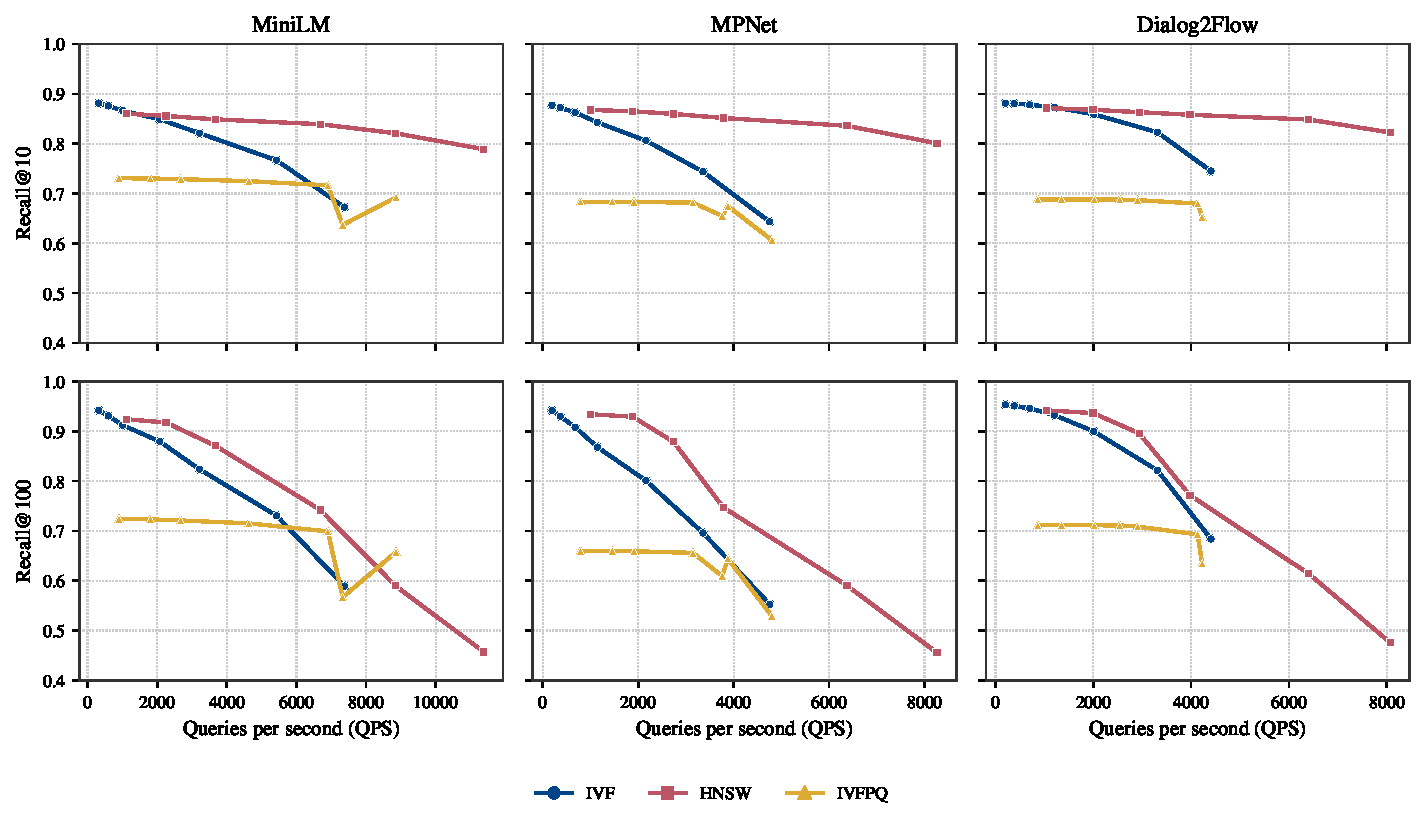
\includegraphics[width=\textwidth]{figures/fig_recall10_recall100_qps_embeddings_independientes.pdf}
\caption{Recall@10 and Recall@100 versus QPS curves for static embeddings.}
\label{fig:recall_qps_static}
\end{figure}

Table~\ref{tab:static_representative} summarizes representative high-recall configurations for IVF and HNSW, together with the exact reference FlatL2 and a configuration compressed via IVFPQ.

\begin{table}[ht]
\centering
\small
\setlength{\tabcolsep}{4pt}
\caption{Approximate retrieval results over static representations.}
\label{tab:static_representative}
\begin{adjustbox}{max width=\textwidth}
\begin{tabular}{llrrrrr}
\toprule
Representation & Index/config. & R@1 & R@10 & R@100 & QPS & Mem. (MB) \\
\midrule
MiniLM & FlatL2 & 1.000 & 1.000 & 1.000 & 62 & 1450.2 \\
MiniLM & IVF $nprobe=64$ & 0.692 & \textbf{0.881} & \textbf{0.942} & 320 & 1463.8 \\
MiniLM & HNSW $efSearch=256$ & 0.674 & 0.860 & 0.924 & \textbf{1115} & 1691.9 \\
MiniLM & IVFPQ $nprobe=64$ & 0.757 & 0.731 & 0.724 & 900 & \textbf{44.1} \\
\midrule
MPNet & FlatL2 & 1.000 & 1.000 & 1.000 & 32 & 2900.5 \\
MPNet & IVF $nprobe=64$ & 0.668 & \textbf{0.877} & \textbf{0.942} & 195 & 2920.0 \\
MPNet & HNSW $efSearch=256$ & 0.660 & 0.868 & 0.934 & \textbf{1001} & 3142.2 \\
MPNet & IVFPQ $nprobe=64$ & 0.730 & 0.683 & 0.660 & 791 & \textbf{50.5} \\
\midrule
Dialog2Flow & FlatL2 & 1.000 & 1.000 & 1.000 & 34 & 2900.5 \\
Dialog2Flow & IVF $nprobe=64$ & 0.685 & \textbf{0.881} & \textbf{0.953} & 203 & 2920.0 \\
Dialog2Flow & HNSW $efSearch=256$ & 0.676 & 0.872 & 0.942 & \textbf{1041} & 3142.2 \\
Dialog2Flow & IVFPQ $nprobe=64$ & 0.730 & 0.688 & 0.711 & 865 & \textbf{50.5} \\
\bottomrule
\end{tabular}
\end{adjustbox}
\end{table}

The results show that dialog2flow-joint-bert-base maintains a competitive behavior compared with the general-purpose sentence embedding models, which indicates that a space specific to conversational flows can be indexed efficiently through ANN methods without substantially degrading the trade-off between retrieval and speed. The Recall@1 > Recall@10 > Recall@100 pattern of IVFPQ, counterintuitive at first glance, arises because Recall@$k$ (the intersection of the $k$ approximate and exact neighbors divided by $k$) is not monotone in $k$, and the nearly identical turns of TOD corpora fall outside the intersection.

A second experimental stage explored the effect of the normalized cumulative variants on the geometry of the vector spaces. Table~\ref{tab:accumulative_geometry} compares each static representation with its cumulative variant through the mean and median cosine similarity between \(e_t\) and \(h_t\), together with the overlap of exact neighbors between the two spaces, making it possible to observe to what extent accumulation modifies the local structure of each base embedding.

\begin{table}[ht]
\centering
\small
\setlength{\tabcolsep}{5pt}
\caption{Geometric comparison between static and cumulative representations.}
\label{tab:accumulative_geometry}
\begin{tabular}{lrrrrr}
\toprule
Base & Mean sim. & Median sim. & Overlap@1 & Overlap@10 & Overlap@100 \\
\midrule
MiniLM & 0.412 & 0.344 & 0.256 & 0.100 & 0.035 \\
MPNet & 0.405 & 0.345 & 0.240 & 0.097 & 0.032 \\
Dialog2Flow & \textbf{0.727} & \textbf{0.702} & \textbf{0.296} & \textbf{0.175} & \textbf{0.152} \\
\bottomrule
\end{tabular}
\end{table}

The results show that the effect of accumulation is not uniform across representations. In MiniLM and MPNet, the similarity between the static and the cumulative representation is around 0.41, with Overlap@100 values close to 0.03, which indicates a substantial modification of the local neighborhood. In contrast, over Dialog2Flow the mean similarity reaches 0.727 and Overlap@100 increases to 0.152, suggesting greater geometric stability with respect to sequential accumulation.

To complement this reading, Figure~\ref{fig:dialog2flow_accumulative} explores the Dialog2Flow space, selected for its specific character for conversational flows and for its competitive behavior in the initial ANN evaluation.

\begin{figure}[ht]
\centering
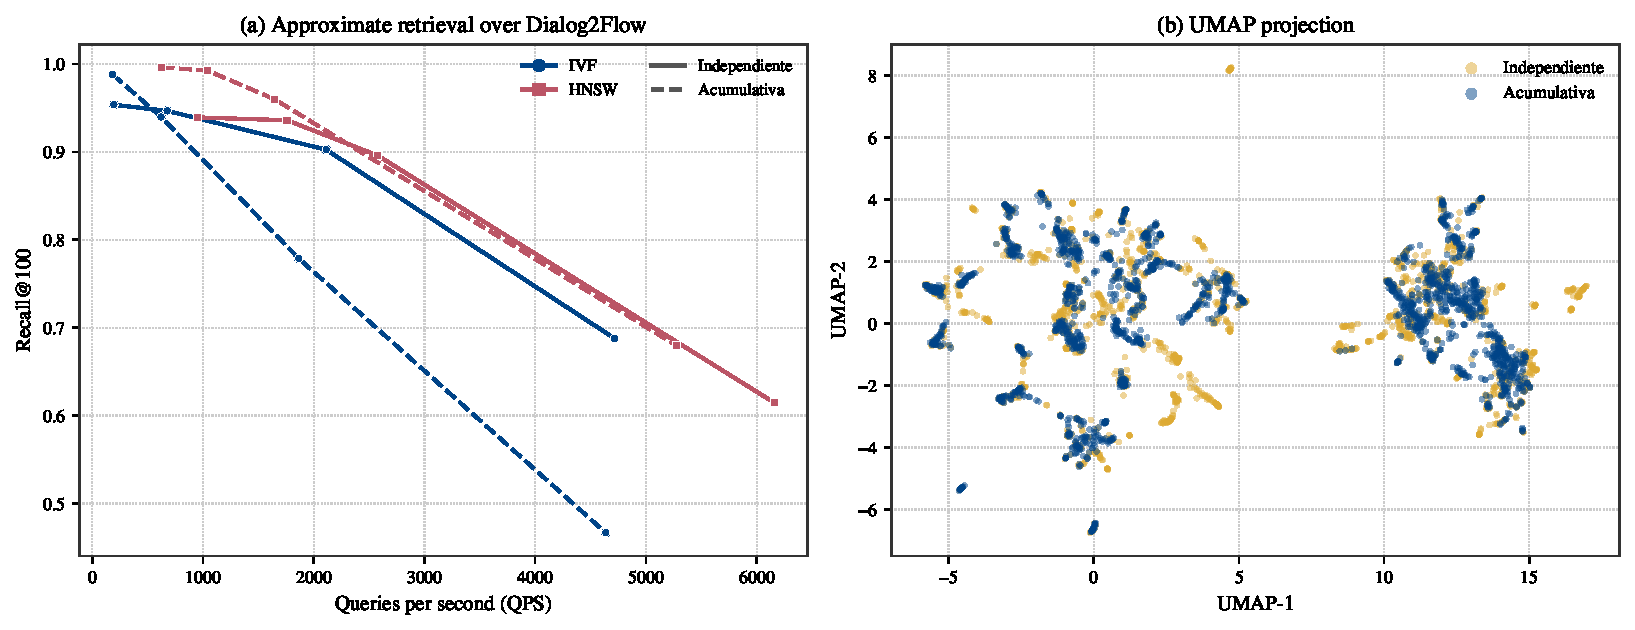
\includegraphics[width=\textwidth]{figures/fig_dialog2flow_independiente_vs_acumulativa_1x2.pdf}
\caption{Exploratory analysis over the Dialog2Flow space.}
\label{fig:dialog2flow_accumulative}
\end{figure}

Figure~\ref{fig:dialog2flow_accumulative} complements the previous geometric analysis through two views of the Dialog2Flow space. In the left panel, the Recall@100 versus QPS curves show that the cumulative variant reaches higher retrieval values than the static representation, both in IVF and in HNSW, especially in configurations with greater exploration. This behavior suggests that sequential accumulation not only modifies the representation, but may also induce a more favorable geometry for approximate search. In the right panel, the UMAP projection reveals a visible reorganization of the space, consistent with the low partial overlap observed between static and cumulative neighborhoods.


In this regard, the third experimental stage aimed to analyze whether the observed geometric differences are reflected in semantic-functionally more plausible neighborhoods. To this end, we applied the LLM-assisted protocol defined in Section~\ref{sec:methodology}, computing MSS@10 for each combination of representation, variant, and ANN index.

Table~\ref{tab:mss_semantic_eval} shows that the cumulative variant achieves its best results when applied over Dialog2Flow. In the three evaluated ANN indexes, cumulative Dialog2Flow obtains the highest MSS@10 values, with scores between 3.65 and 3.67 on a scale from 1 to 5. In contrast, accumulation over the general-purpose models MiniLM and MPNet does not produce an equivalent improvement: their cumulative variants show values slightly lower than the static representations in the three indexes.

\begin{table}[ht]
\centering
\small
\setlength{\tabcolsep}{5pt}
\caption{Semantic-functional evaluation of retrieved neighbors. MSS@10 is reported together with the standard deviation across queries.}
\label{tab:mss_semantic_eval}
\begin{tabular}{llrrr}
\toprule
Representation & Variant & IVF & HNSW & IVFPQ \\
\midrule
MiniLM & Static & 3.399 $\pm$ 0.758 & 3.416 $\pm$ 0.741 & 3.346 $\pm$ 0.803 \\
MiniLM & Cumulative & 3.315 $\pm$ 0.754 & 3.334 $\pm$ 0.758 & 3.234 $\pm$ 0.769 \\
\midrule
MPNet & Static & 3.381 $\pm$ 0.773 & 3.358 $\pm$ 0.803 & 3.368 $\pm$ 0.819 \\
MPNet & Cumulative & 3.309 $\pm$ 0.776 & 3.310 $\pm$ 0.761 & 3.197 $\pm$ 0.742 \\
\midrule
Dialog2Flow & Static & 3.294 $\pm$ 0.803 & 3.293 $\pm$ 0.767 & 3.296 $\pm$ 0.742 \\
Dialog2Flow & Cumulative & \textbf{3.665 $\pm$ 0.588} & \textbf{3.661 $\pm$ 0.581} & \textbf{3.647 $\pm$ 0.629} \\
\bottomrule
\end{tabular}
\end{table}

To analyze whether the improvement of cumulative Dialog2Flow depended on a few extreme cases, a paired per-query comparison was carried out between the static and cumulative variants. Table~\ref{tab:paired_semantic_eval} reports the percentage of queries in which the cumulative variant obtained a higher SS@10 value than the static variant.

\begin{table}[ht]
\centering
\small
\setlength{\tabcolsep}{6pt}
\caption{Percentage of queries in which the cumulative variant outperforms the static one according to SS@10.}
\label{tab:paired_semantic_eval}
\begin{tabular}{lrrr}
\toprule
Representation & IVF & HNSW & IVFPQ \\
\midrule
MiniLM & 47\% & 48\% & 44\% \\
MPNet & 48\% & 48\% & 41\% \\
Dialog2Flow & \textbf{68\%} & \textbf{65\%} & \textbf{68\%} \\
\bottomrule
\end{tabular}
\end{table}

The paired comparison reinforces the previous interpretation. In Dialog2Flow, the cumulative variant outperforms the static one in the majority of queries for the three evaluated indexes, with values between 65\% and 68\%. In contrast, for MiniLM and MPNet, the percentages remain close to parity or below 50\%. This suggests that the improvement observed in Dialog2Flow does not depend only on extreme values, but is distributed over a majority proportion of queries.

As a final experimental stage, we evaluated whether the previous normalized cumulative representation over Dialog2Flow could be improved by replacing the uniform accumulation scheme with the exponential moving average (EMA) defined in Eq.~(\ref{eq:ema}), sweeping $\alpha \in \{0.1,0.2,\ldots,0.9\}$. This experiment was restricted to Dialog2Flow, since the previous semantic-functional evaluation showed that this was the only representation space in which sequential accumulation produced a clear improvement.

Figure~\ref{fig:visual-ema2} shows a clear sensitivity of the semantic-functional performance to the EMA parameter. Low values of $\alpha$ underperform the previous dynamic baseline, suggesting that excessive historical inertia harms the retrieved neighborhoods. 


\begin{figure}[ht]
\centering
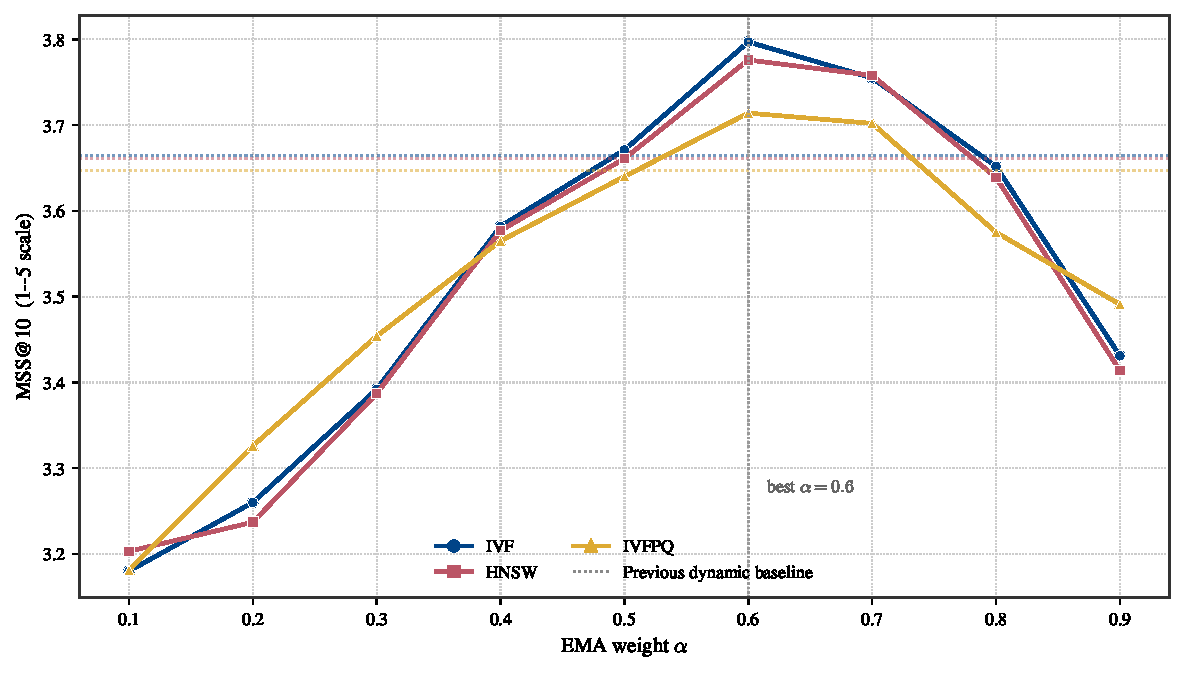
\includegraphics[width=0.63\textwidth]{figures/visual-ema-2.pdf}
\caption{MSS@10 as a function of the EMA parameter $\alpha$ across ANN indices.}
\label{fig:visual-ema2}
\end{figure}

Conversely, intermediate values improve over the previous dynamic representation, with the best performance obtained at $\alpha=0.6$ for the three ANN indexes. The previous dynamic representation is closely related to the EMA formulation with $\alpha=0.5$, since both assign symmetric weight to the previous state and the current turn before applying normalization. Although they are not strictly identical due to normalization and numerical details, their MSS@10 values are nearly equivalent, which supports the consistency of the EMA sweep.

Table~\ref{tab:ema_vs_dynamic_per_query} complements the aggregate MSS@10 results with a paired query-level comparison against the previous dynamic baseline for each index.

\begin{table}[ht]
\centering
\scriptsize
\setlength{\tabcolsep}{3.5pt}
\renewcommand{\arraystretch}{1.12}
\caption{Per-query comparison of EMA-based Dialog2Flow representations against the previous dynamic baseline. W/T/L denotes wins, ties, and losses over the 100 paired queries.}
\label{tab:ema_vs_dynamic_per_query}
\begin{adjustbox}{max width=\textwidth}
\begin{tabular}{c rrc rrc rrc}
\toprule
\multirow{2}{*}{$\boldsymbol{\alpha}$} &
\multicolumn{3}{c}{\textbf{IVF} $(3.665)$} &
\multicolumn{3}{c}{\textbf{HNSW} $(3.661)$} &
\multicolumn{3}{c}{\textbf{IVFPQ} $(3.647)$} \\
\cmidrule(lr){2-4}
\cmidrule(lr){5-7}
\cmidrule(lr){8-10}
& \textbf{MSS} & $\boldsymbol{\Delta}$ & \textbf{W/T/L}
& \textbf{MSS} & $\boldsymbol{\Delta}$ & \textbf{W/T/L}
& \textbf{MSS} & $\boldsymbol{\Delta}$ & \textbf{W/T/L} \\
\midrule
0.1 & 3.180 & -0.485 & 29/6/65  & 3.203 & -0.458 & 23/12/65 & 3.181 & -0.466 & 28/7/65  \\
0.2 & 3.260 & -0.405 & 25/11/64 & 3.237 & -0.424 & 24/8/68  & 3.326 & -0.321 & 33/11/56 \\
0.3 & 3.392 & -0.273 & 29/9/62  & 3.387 & -0.274 & 30/12/58 & 3.454 & -0.193 & 36/9/55  \\
0.4 & 3.582 & -0.083 & 37/11/52 & 3.577 & -0.084 & 35/16/49 & 3.565 & -0.082 & 35/10/55 \\
0.5 & 3.671 & +0.006 & 26/54/20 & 3.661 & +0.000 & 22/54/24 & 3.640 & -0.007 & 38/19/43 \\
\textbf{0.6}
    & \textbf{3.797} & \textbf{+0.132} & \textbf{52/17/31}
    & \textbf{3.776} & \textbf{+0.115} & \textbf{45/17/38}
    & \textbf{3.714} & \textbf{+0.067} & \textbf{45/17/38} \\
0.7 & 3.755 & +0.090 & 49/15/36 & 3.758 & +0.097 & 46/15/39 & 3.702 & +0.055 & 48/14/38 \\
0.8 & 3.652 & -0.013 & 38/13/49 & 3.639 & -0.022 & 40/14/46 & 3.575 & -0.072 & 38/15/47 \\
0.9 & 3.431 & -0.234 & 33/9/58  & 3.414 & -0.247 & 32/8/60  & 3.491 & -0.156 & 35/15/50 \\
\bottomrule
\end{tabular}
\end{adjustbox}
\end{table}

The best EMA configuration, $\alpha=0.6$, improves over the dynamic baseline by $+0.132$ in IVF, $+0.115$ in HNSW, and $+0.067$ in IVFPQ. Moreover, the win/tie/loss counts indicate that this improvement is not explained only by a few extreme scores: for IVF, EMA with $\alpha=0.6$ obtains a higher SS@10 in 52 queries, ties in 17, and loses in 31; for HNSW and IVFPQ, it also produces more wins than losses. A similar, although slightly weaker, pattern is observed for $\alpha=0.7$.

To assess whether these gains could be attributed to retrieving nearby turns from the same conversation, we conducted an additional same-dialogue neighbor analysis. This check is relevant because the query/index split was performed at the vector level: although a query cannot retrieve its own vector, other turns from the same dialogue may still be present in the index. 

\begin{table}[ht]
\centering
\scriptsize
\setlength{\tabcolsep}{4pt}
\renewcommand{\arraystretch}{1.12}
\caption{Same-dialogue neighbor analysis over Dialog2Flow}
\label{tab:same_dialogue_analysis}
\begin{adjustbox}{max width=\textwidth}
\begin{tabular}{llrrrrr}
\toprule
\textbf{Representation} & \textbf{Index} & \textbf{MSS@10} & \textbf{Same@10} & \textbf{Q-Same} & \textbf{Same score} & \textbf{Cross score} \\
\midrule
Static D2F & IVF   & 3.294 & 0.0\%  & 0.0\%  & --    & 3.294 \\
Static D2F & HNSW  & 3.293 & 0.0\%  & 0.0\%  & --    & 3.293 \\
Static D2F & IVFPQ & 3.296 & 0.0\%  & 0.0\%  & --    & 3.296 \\
\midrule
Dynamic D2F & IVF   & 3.665 & 23.1\% & 93.0\% & 3.823 & 3.618 \\
Dynamic D2F & HNSW  & 3.661 & 23.2\% & 93.0\% & 3.862 & 3.600 \\
Dynamic D2F & IVFPQ & 3.647 & 14.4\% & 74.0\% & 4.021 & 3.584 \\
\midrule
EMA D2F ($\alpha=0.6$) & IVF   & \textbf{3.797} & 12.9\% & 72.0\% & 4.186 & \textbf{3.739} \\
EMA D2F ($\alpha=0.6$) & HNSW  & \textbf{3.776} & 12.9\% & 71.0\% & 4.140 & \textbf{3.722} \\
EMA D2F ($\alpha=0.6$) & IVFPQ & \textbf{3.714} & 6.2\%  & 47.0\% & 4.065 & \textbf{3.691} \\
\bottomrule
\end{tabular}
\end{adjustbox}
\end{table}

The uniform dynamic representation retrieves a non-negligible proportion of same-dialogue neighbors, reaching 23.1\% and 23.2\% of the top-10 results for IVF and HNSW, respectively. However, this effect does not explain the EMA improvement: the best EMA configuration ($\alpha=0.6$) reduces the same-dialogue proportion to 12.9\% for both IVF and HNSW, and to 6.2\% for IVFPQ, while still achieving the highest MSS@10. Moreover, when considering only cross-dialogue neighbor pairs, EMA with $\alpha=0.6$ remains above the previous dynamic baseline across the three indexes. Therefore, the observed improvement of the calibrated EMA representation cannot be attributed solely to intra-dialogue continuity.

The same-dialogue analysis above is computed \emph{post hoc}: neighbors are first retrieved and only afterwards partitioned into same- and cross-dialogue pairs. While this already indicates that the EMA gain is not a by-product of intra-dialogue continuity, it does not control the retrieval process itself, since the indexes still return same-dialogue turns that are merely relabelled after the fact. To place every variant on a strictly cross-dialogue footing, we re-evaluated the static representation, the uniform dynamic baseline, and the calibrated EMA ($\alpha=0.6$) under the cross-dialogue filtered protocol of Section~\ref{sec:crossdlg_protocol}, which removes same-dialogue neighbors at query time and adds $400$ held-out queries as an out-of-sample confirmation of the calibrated setting.

Figure~\ref{fig:crossdlg_overview} reports MSS@10 under this stricter protocol, showing the mean for each variant and index with $95\%$ confidence intervals together with the static$\,\rightarrow\,$dynamic$\,\rightarrow\,$EMA progression. The ordering observed in the previous stages is preserved once all retrieval is forced to be cross-dialogue: the static representation stays around $3.35$, the uniform dynamic baseline rises to $3.69$--$3.74$, and the calibrated EMA attains the highest values, $3.77$--$3.80$, across the three indexes.

\iffalse  % removed from body to avoid redundancy with the overview figure (Fig. crossdlg_overview); kept here, not deleted -- no numbers lost
\begin{table}[ht]
\centering
\small
\setlength{\tabcolsep}{6pt}
\caption{Cross-dialogue filtered semantic-functional evaluation over Dialog2Flow. Same-dialogue neighbors are removed at query time, and MSS@10 is reported together with the standard deviation across $n=500$ queries (the original $100$ plus $400$ held-out).}
\label{tab:crossdlg_mss}
\begin{tabular}{lrrr}
\toprule
Variant & IVF & HNSW & IVFPQ \\
\midrule
Static & 3.353 $\pm$ 0.751 & 3.360 $\pm$ 0.740 & 3.342 $\pm$ 0.746 \\
Dynamic & 3.719 $\pm$ 0.643 & 3.738 $\pm$ 0.635 & 3.690 $\pm$ 0.619 \\
EMA ($\alpha=0.6$) & \textbf{3.802 $\pm$ 0.658} & \textbf{3.804 $\pm$ 0.652} & \textbf{3.765 $\pm$ 0.669} \\
\bottomrule
\end{tabular}
\end{table}
\fi

\begin{figure}[ht]
\centering
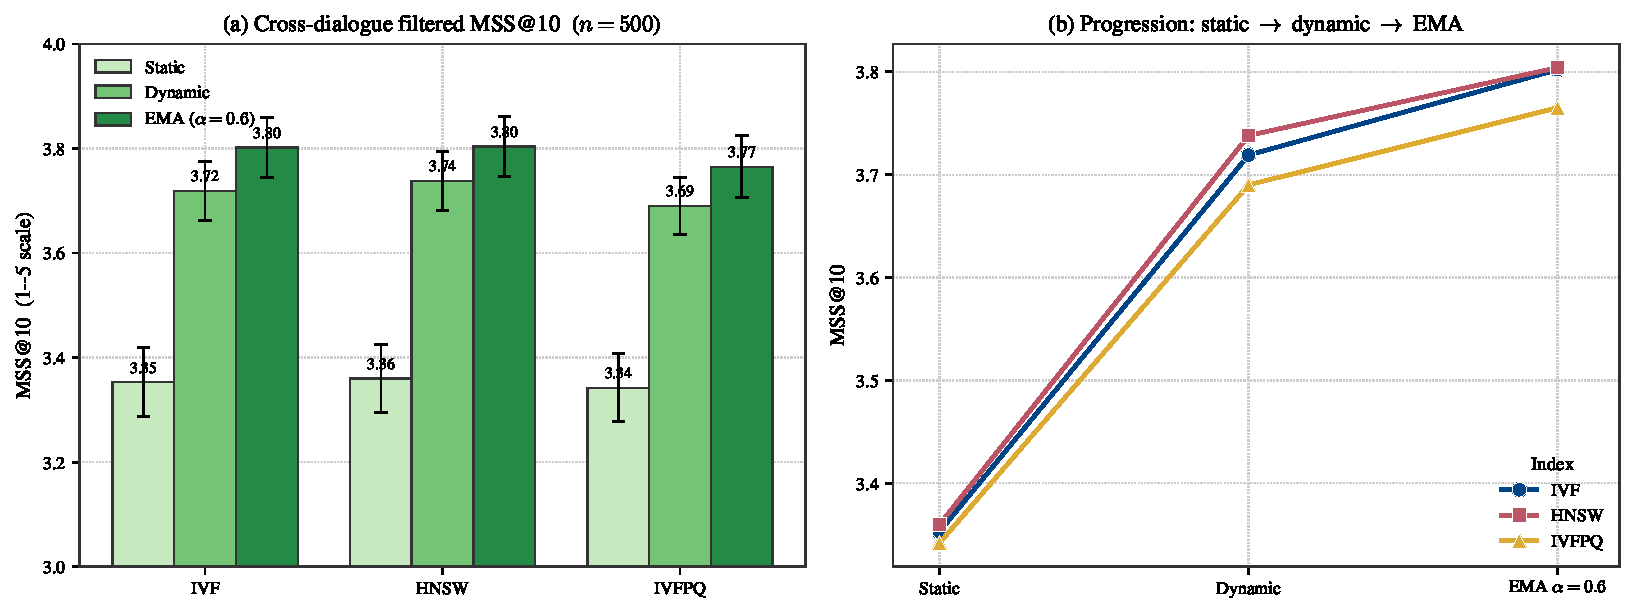
\includegraphics[width=\textwidth]{figures/fig_crossdlg_overview.pdf}
\caption{Cross-dialogue filtered MSS@10 over Dialog2Flow ($n=500$): (a) mean per variant and index ($95\%$ CIs); (b) the static$\,\rightarrow\,$dynamic$\,\rightarrow\,$EMA progression.}
\label{fig:crossdlg_overview}
\end{figure}

Table~\ref{tab:crossdlg_wilcoxon} reports the paired signed-rank tests, and two results stand out. First, the central static-to-dynamic effect survives the cross-dialogue filter with a wide margin: $\Delta\approx0.35$--$0.38$ with $p$-values between $10^{-23}$ and $10^{-25}$ on the full set, and still between $10^{-18}$ and $10^{-19}$ on the $400$ held-out queries, in every index. Second, and most importantly, the calibrated EMA update now \emph{significantly} outperforms the uniform dynamic baseline in all three indexes---a contrast that was only borderline ($p\approx0.06$) in the earlier $n=100$ evaluation. Crucially, the same holds on the held-out queries (right-hand columns of Table~\ref{tab:crossdlg_wilcoxon}): EMA $-$ Dynamic yields $\Delta=+0.085$ ($p=7.0\times10^{-5}$) for IVF, $+0.066$ ($p=7.7\times10^{-4}$) for HNSW, and $+0.079$ ($p=1.2\times10^{-3}$) for IVFPQ. Because these queries played no part in choosing $\alpha=0.6$, this is an out-of-sample confirmation of the calibrated setting and removes any concern that $\alpha$ might have been selected and evaluated on the same sample.

\begin{table}[ht]
\centering
\scriptsize
\setlength{\tabcolsep}{5pt}
\renewcommand{\arraystretch}{1.1}
\caption{Paired Wilcoxon signed-rank tests on the cross-dialogue filtered MSS@10. $\Delta$: mean per-query difference; $p$: two-sided value. \emph{Full}: all $500$ queries; \emph{Held-out}: the $400$ not used to select $\alpha=0.6$.}
\label{tab:crossdlg_wilcoxon}
\begin{adjustbox}{max width=\textwidth}
\begin{tabular}{ll rr rr}
\toprule
\multirow{2}{*}{Contrast} & \multirow{2}{*}{Index} & \multicolumn{2}{c}{Full ($n=500$)} & \multicolumn{2}{c}{Held-out ($n=400$)} \\
\cmidrule(lr){3-4}\cmidrule(lr){5-6}
 & & $\Delta$ & $p$ & $\Delta$ & $p$ \\
\midrule
\multirow{3}{*}{Dynamic $-$ Static}
 & IVF   & $+0.366$ & $8.8\times10^{-25}$ & $+0.357$ & $1.1\times10^{-19}$ \\
 & HNSW  & $+0.378$ & $2.2\times10^{-25}$ & $+0.364$ & $1.3\times10^{-19}$ \\
 & IVFPQ & $+0.349$ & $2.2\times10^{-23}$ & $+0.347$ & $5.8\times10^{-18}$ \\
\midrule
\multirow{3}{*}{EMA $-$ Dynamic}
 & IVF   & $+0.083$ & $1.6\times10^{-5}$  & $+0.085$ & $7.0\times10^{-5}$ \\
 & HNSW  & $+0.066$ & $4.2\times10^{-4}$  & $+0.066$ & $7.7\times10^{-4}$ \\
 & IVFPQ & $+0.074$ & $5.2\times10^{-4}$  & $+0.079$ & $1.2\times10^{-3}$ \\
\midrule
\multirow{3}{*}{EMA $-$ Static}
 & IVF   & $+0.449$ & $1.8\times10^{-34}$ & $+0.442$ & $4.7\times10^{-27}$ \\
 & HNSW  & $+0.444$ & $9.8\times10^{-35}$ & $+0.430$ & $2.0\times10^{-26}$ \\
 & IVFPQ & $+0.423$ & $1.4\times10^{-32}$ & $+0.426$ & $3.2\times10^{-26}$ \\
\bottomrule
\end{tabular}
\end{adjustbox}
\end{table}

\iffalse  % removed from body to avoid redundancy with the Wilcoxon table (Table crossdlg_wilcoxon); kept here, not deleted -- no numbers lost
\begin{figure}[ht]
\centering
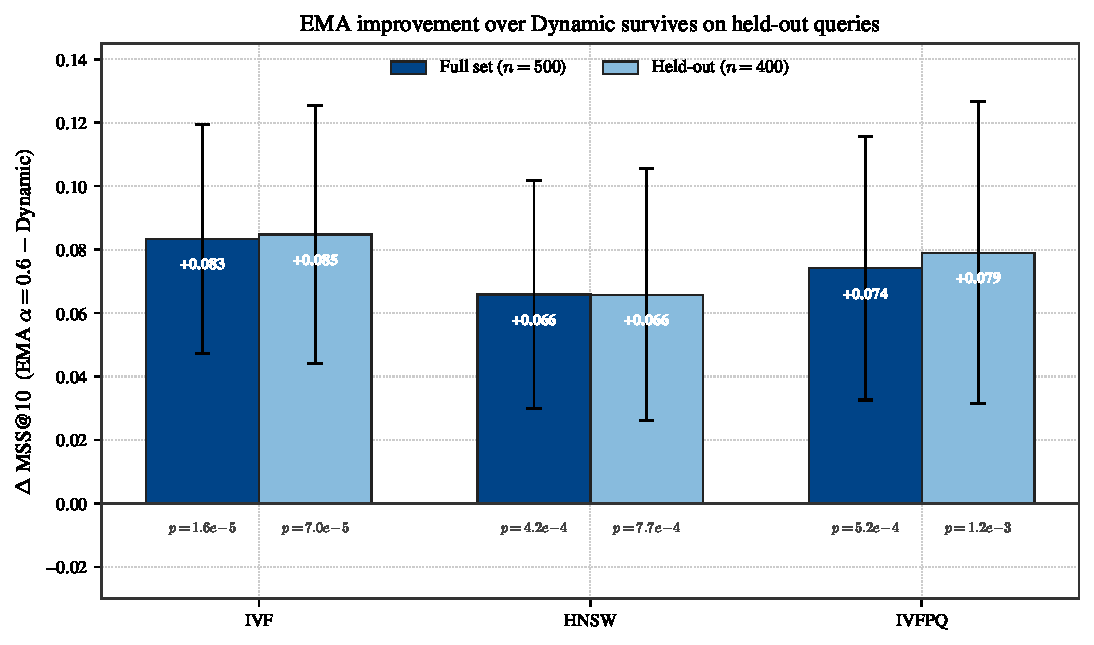
\includegraphics[width=0.85\textwidth]{figures/fig_crossdlg_ema_confirmation.pdf}
\caption{Improvement of the calibrated EMA ($\alpha=0.6$) over the uniform dynamic baseline in MSS@10, with $95\%$ confidence intervals and Wilcoxon $p$-values. The effect is positive and significant for every index, on both the full set and the $400$ held-out queries.}
\label{fig:crossdlg_ema_confirmation}
\end{figure}
\fi

\iffalse  % removed from body to avoid redundancy with the near-duplicate figure (Fig. crossdlg_nearduplicates); kept here, not deleted -- no numbers lost
\begin{table}[ht]
\centering
\small
\setlength{\tabcolsep}{6pt}
\caption{Cross-dialogue near-duplicates: textually near-identical turns drawn from \emph{other} dialogues. Near-dup@10 is the percentage of retained top-$10$ neighbors flagged as near-duplicates; Rank-1 is the percentage of queries whose nearest neighbor is a near-duplicate.}
\label{tab:crossdlg_neardup}
\begin{tabular}{lrr}
\toprule
Variant & Near-dup@10 & Rank-1 near-dup \\
\midrule
Static & 16.4\% & 43.2\% \\
Dynamic & 3.8\% & 20.8\% \\
EMA ($\alpha=0.6$) & 3.8\% & 20.9\% \\
\bottomrule
\end{tabular}
\end{table}
\fi

Finally, the query-time filter brought to light a phenomenon that the previous stages could not isolate. Because only the \texttt{dialogue\_id} filter is applied, textually near-identical turns that recur across \emph{different} dialogues---a known property of the underlying task-oriented corpora---remain in the index and can still be retrieved. Figure~\ref{fig:crossdlg_nearduplicates} shows that the static representation retrieves these cross-dialogue near-duplicates far more often than the dynamic variants: they account for $16.4\%$ of its top-$10$ neighbors, and the nearest neighbor is a near-duplicate for $43.2\%$ of queries, against only $3.8\%$ of neighbors and roughly $21\%$ of queries for both the dynamic and the EMA representations. Since near-duplicate pairs receive markedly higher judge scores (mean overall similarity $4.18$ versus $3.57$), this asymmetry \emph{inflates} the static MSS@10 upward; the static-to-dynamic gap reported above is therefore a conservative estimate of the true advantage of cumulative representations. The EMA $-$ Dynamic contrast, in turn, is unaffected, as both variants retain near-identical near-duplicate rates ($3.77\%$ versus $3.79\%$); restricting the comparison to non-near-duplicate neighbors leaves it essentially unchanged (IVF: $\Delta=+0.086$, $p=1.8\times10^{-5}$). Beyond its role as a control, this asymmetry is itself interpretable: the static space over-retrieves surface-level lexical repetitions drawn from unrelated dialogues, whereas the cumulative and calibrated representations favor neighbors that are functionally, rather than merely textually, similar.

\begin{figure}[ht]
\centering
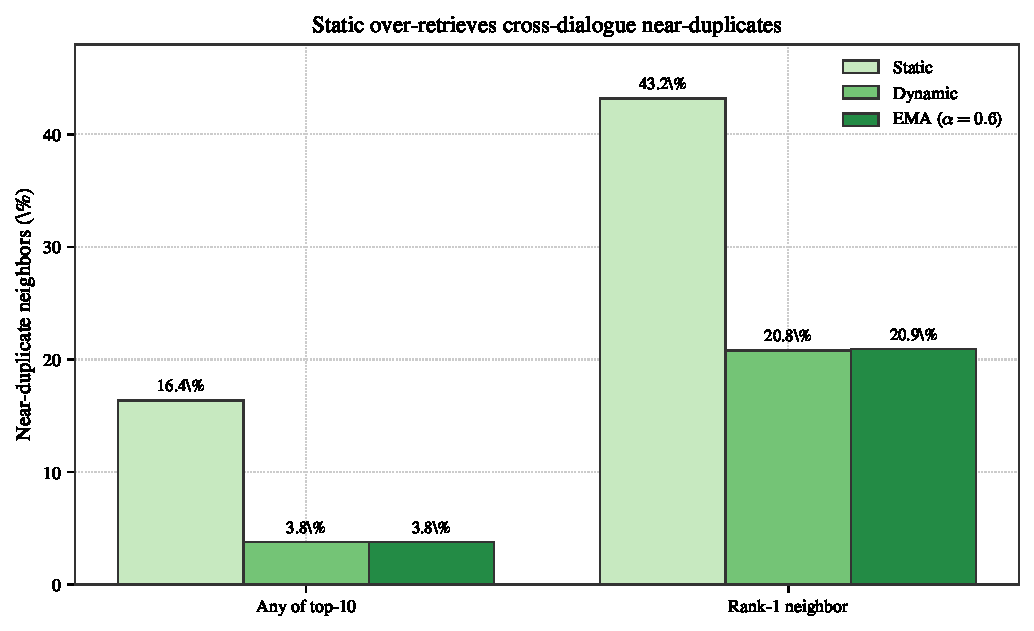
\includegraphics[width=0.8\textwidth]{figures/fig_crossdlg_nearduplicates.pdf}
\caption{Cross-dialogue near-duplicate retrieval by variant (Near-dup@10 and rank-1 rates).}
\label{fig:crossdlg_nearduplicates}
\end{figure}



Taken together, these results indicate that normalized sequential accumulation does not constitute a universal improvement over any embedding space. Its effect depends on the base space: in the general-purpose models it modifies the neighborhood without improving its semantic-functional plausibility, whereas in Dialog2Flow it induces more favorable neighborhoods both from a geometric and a semantic-functional point of view. The EMA sweep further shows that the previous dynamic representation can be improved by calibrating the balance between conversational history and the current turn, with the most favorable results obtained around $\alpha=0.6$. The same-dialogue analysis also shows that this improvement is not merely a by-product of retrieving neighboring turns from the same conversation: the best EMA setting reduces the proportion of same-dialogue neighbors with respect to the uniform dynamic baseline while maintaining higher semantic-functional scores. A final cross-dialogue \emph{filtered} re-evaluation on $500$ queries---including $400$ held-out queries that played no role in selecting $\alpha$---confirms this picture under a stricter protocol: the static-to-dynamic gain remains significant at $p<10^{-17}$ in every index, and the calibrated $\alpha=0.6$ update significantly outperforms the uniform dynamic baseline precisely on the held-out queries (Wilcoxon $p<1.3\times10^{-3}$), resolving the borderline result of the earlier $n=100$ comparison.


\section{Conclusions and future work}
\label{sec:conclusions}

In this work we studied approximate nearest neighbor search over static, normalized cumulative, and EMA-based embeddings for conversational memory in task-oriented dialogue. Based on a collection of 101{,}021 dialogues and 1{,}000{,}023 turns derived from Dialog2Flow, we evaluated three representation spaces and the IVF, HNSW, and IVFPQ indexes implemented in FAISS.

The results show that ANN methods retrieve conversational representations at scale with controllable trade-offs among recall, QPS, and memory. HNSW presented a favorable balance between retrieval and speed, while IVFPQ substantially reduced memory at the cost of a loss in recall. These results support the feasibility of using ANN indexes as an efficient retrieval layer for conversational memory.

The central contribution emerges from the comparison between static and dynamic representations. The normalized cumulative representation did not provide a uniform improvement over the general-purpose MiniLM and MPNet spaces. In contrast, when applied over Dialog2Flow, it produced more favorable neighborhoods from both a geometric and a semantic-functional point of view, outperforming the static variant in most of the evaluated queries.

The EMA analysis further refines this result. Instead of treating accumulation as a fixed uniform update, the EMA formulation explicitly controls the balance between the accumulated conversational history and the current turn. The best results were obtained with $\alpha=0.6$, consistently across IVF, HNSW, and IVFPQ, improving over the previous dynamic Dialog2Flow baseline. The per-query win/tie/loss comparison also suggests that this improvement is not explained only by a small number of extreme cases, but by a broader shift in retrieval quality around the optimal weighting region. In addition, the same-dialogue neighbor analysis indicates that the best EMA configuration reduces intra-dialogue retrieval with respect to the uniform dynamic baseline, suggesting that its gains are not solely due to retrieving adjacent turns from the same conversation. A subsequent cross-dialogue filtered re-evaluation, in which same-dialogue neighbors are removed at query time and the calibrated setting is tested on a disjoint set of $400$ held-out queries, confirms that the $\alpha=0.6$ update significantly outperforms the uniform dynamic baseline across the three indexes (Wilcoxon $p<1.3\times10^{-3}$), ruling out same-dialogue retrieval as an explanation of the gain.

Taken together, these results suggest that the usefulness of cumulative representations depends on the geometry of the base space and on the update policy used to incorporate conversational history. A simple accumulation may not be sufficient over general-purpose embeddings; however, when applied over a representation space oriented toward dialogue-flow regularities, both uniform accumulation and calibrated EMA updates can induce more useful neighborhoods for conversational memory.

As future work, a natural continuation is to move from post-hoc accumulation policies toward learned contextual turn embeddings. In this direction, each turn representation would be produced as a function not only of the turn itself, but also of its conversational context. This could be explored under two complementary settings: a bidirectional formulation, where the representation of a turn is conditioned on the complete dialogue, and an autoregressive formulation, where it is conditioned only on the preceding turns. In this sense, the goal is analogous to contextual token representations in language models, but operating at the level of dialogue turns rather than tokens. Such models could learn richer update functions than uniform accumulation or EMA, potentially incorporating speaker roles, dialogue acts, slots, intents, and task-flow information. It is also relevant to evaluate these representations on concrete task-oriented dialogue tasks, such as next-action selection, missing-information detection, or recommendation of conversational trajectories.

\bibliographystyle{splncs04}
\bibliography{References}

\end{document}
